\documentclass[tikz,border=10pt]{standalone}
\usepackage[T1]{fontenc}
\usepackage{lmodern}
\usepackage{amsmath}
\usepackage{amssymb}
\usetikzlibrary{arrows.meta,positioning,calc,shapes.geometric,shadows,fit,backgrounds}

\definecolor{InputBlue}{HTML}{1F77B4}
\definecolor{FormulaGreen}{HTML}{2CA02C}
\definecolor{DeltaOrange}{HTML}{FF7F0E}
\definecolor{RuleTeal}{HTML}{007C89}
\definecolor{OutputPurple}{HTML}{9467BD}
\definecolor{Ink}{HTML}{1F2937}
\definecolor{SoftGray}{HTML}{F7F8FA}
\definecolor{LineGray}{HTML}{6B7280}

\begin{document}
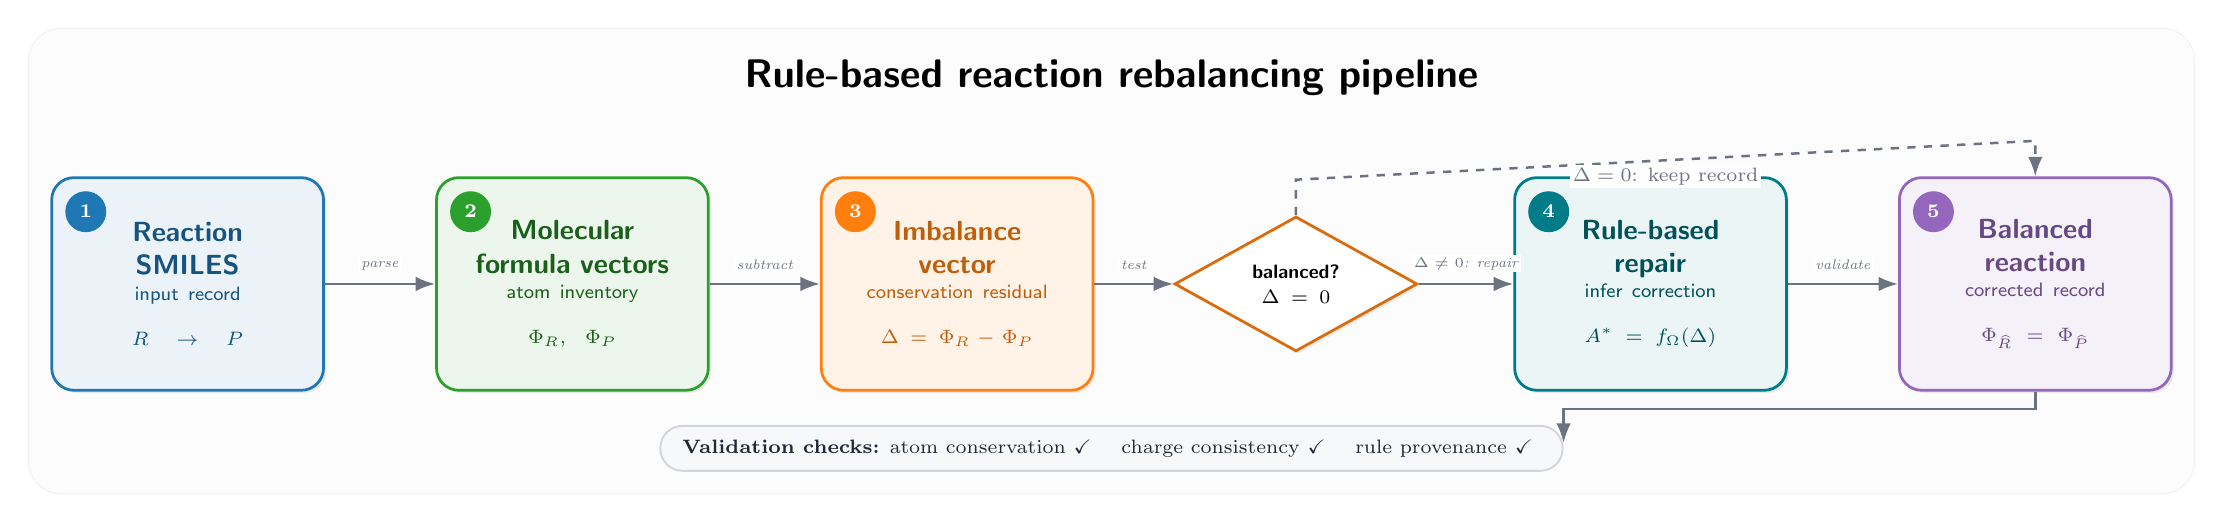
\begin{tikzpicture}[
  font=\sffamily,
  >=Latex,
  title/.style={font=\sffamily\bfseries\Large, text=black, align=center},
  subtitle/.style={font=\sffamily\small, text=LineGray, align=center},
  stage/.style={
    rounded corners=8pt,
    minimum height=27mm,
    text width=31mm,
    align=center,
    line width=1pt,
    inner sep=5pt,
    drop shadow={shadow xshift=1.0pt, shadow yshift=-1.0pt, opacity=0.16}
  },
  stepbadge/.style={
    circle,
    minimum size=5.2mm,
    inner sep=0pt,
    font=\bfseries\scriptsize,
    text=white
  },
  arrow/.style={-Latex, line width=0.9pt, draw=LineGray},
  bypass/.style={-Latex, line width=0.9pt, draw=LineGray, dashed},
  edgelabel/.style={midway, above=1.3mm, font=\tiny\itshape, text=LineGray, fill=white, inner sep=1pt},
  smallnote/.style={font=\scriptsize, text=LineGray, align=center, fill=white, inner sep=1pt},
  qc/.style={
    rounded corners=8pt,
    draw=LineGray!30,
    fill=SoftGray,
    line width=0.7pt,
    font=\scriptsize,
    text=Ink,
    align=center,
    inner xsep=8pt,
    inner ysep=5pt
  }
]

% ---------- Main stages ----------
\node[stage, draw=InputBlue, fill=InputBlue!9, text=InputBlue!70!black] (input) at (0,0) {
  \textbf{Reaction\\SMILES}\\[-1mm]
  {\scriptsize input record}\\[1.5mm]
  {\scriptsize $R \;\rightarrow\; P$}
};
\node[stepbadge, fill=InputBlue] at ($(input.north west)+(4.5mm,-4.5mm)$) {1};

\node[stage, draw=FormulaGreen, fill=FormulaGreen!9, text=FormulaGreen!60!black, right=14mm of input] (formula) {
  \textbf{Molecular\\formula vectors}\\[-1mm]
  {\scriptsize atom inventory}\\[1.5mm]
  {\scriptsize $\Phi_R,\;\Phi_P$}
};
\node[stepbadge, fill=FormulaGreen] at ($(formula.north west)+(4.5mm,-4.5mm)$) {2};

\node[stage, draw=DeltaOrange, fill=DeltaOrange!10, text=DeltaOrange!75!black, right=14mm of formula] (delta) {
  \textbf{Imbalance\\vector}\\[-1mm]
  {\scriptsize conservation residual}\\[1.5mm]
  {\scriptsize $\Delta = \Phi_R - \Phi_P$}
};
\node[stepbadge, fill=DeltaOrange] at ($(delta.north west)+(4.5mm,-4.5mm)$) {3};

\node[diamond, aspect=1.8, draw=DeltaOrange!85!black, fill=white, line width=1pt,
      text width=20mm, align=center, right=10mm of delta, inner sep=1pt,
      drop shadow={shadow xshift=1pt, shadow yshift=-1pt, opacity=0.12}] (decision)
      {\scriptsize\bfseries balanced?\\[-1mm]$\Delta=0$};

\node[stage, draw=RuleTeal, fill=RuleTeal!8, text=RuleTeal!65!black, right=12mm of decision] (repair) {
  \textbf{Rule-based\\repair}\\[-1mm]
  {\scriptsize infer correction}\\[1.5mm]
  {\scriptsize $A^{\ast}=f_{\Omega}(\Delta)$}
};
\node[stepbadge, fill=RuleTeal] at ($(repair.north west)+(4.5mm,-4.5mm)$) {4};

\node[stage, draw=OutputPurple, fill=OutputPurple!9, text=OutputPurple!70!black, right=14mm of repair] (output) {
  \textbf{Balanced\\reaction}\\[-1mm]
  {\scriptsize corrected record}\\[1.5mm]
  {\scriptsize $\Phi_{\widehat R}=\Phi_{\widehat P}$}
};
\node[stepbadge, fill=OutputPurple] at ($(output.north west)+(4.5mm,-4.5mm)$) {5};

% ---------- Title ----------
\node[title] (heading) at ($(input.north west)!0.5!(output.north east)+(0,1.25)$)
  {Rule-based reaction rebalancing pipeline};
% ---------- Edges ----------
\draw[arrow] (input) -- node[edgelabel] {parse} (formula);
\draw[arrow] (formula) -- node[edgelabel] {subtract} (delta);
\draw[arrow] (delta) -- node[edgelabel] {test} (decision);
\draw[arrow] (decision) -- node[edgelabel] {$\Delta\neq0$: repair} (repair);
\draw[arrow] (repair) -- node[edgelabel] {validate} (output);

\coordinate (yesA) at ($(decision.north)+(0,0.45)$);
\coordinate (yesB) at ($(output.north)+(0,0.45)$);
\draw[bypass] (decision.north) -- (yesA) -- node[smallnote, below=0.5mm] {$\Delta=0$: keep record} (yesB) -- (output.north);

% ---------- Audit layer ----------
\coordinate (qcpos) at ($(formula.south)!0.50!(repair.south)+(0,-0.72)$);
\node[qc] (qcbox) at (qcpos) {
  \textbf{Validation checks:} atom conservation $\checkmark$ \quad charge consistency $\checkmark$ \quad rule provenance $\checkmark$
};
\draw[arrow, shorten >=2pt] (output.south) -- ++(0,-0.22) -| (qcbox.east);

% ---------- Background grouping ----------
\begin{scope}[on background layer]
  \node[fit=(input)(formula)(delta)(decision)(repair)(output)(qcbox)(heading),
        rounded corners=12pt,
        fill=black!1,
        draw=black!5,
        inner sep=8pt] {};
\end{scope}

\end{tikzpicture}
\end{document}
